\chapter{Organisation du projet}

	\section{Gestion du projet}

		Afin de faciliter la communication et le bon déroulement de la conception de notre application, divers moyens ont été mis en œuvre.

		\subsection{Gestionnaire de version}

			Tout d'abord, nous pouvons citer l'utilisation d'un gestionnaire de version afin de permettre la centralisation du code et rendre le travail en équipe bien plus efficace. Le choix de celui-ci étant imposé (\textit{Subversion}), il n'est pas nécessaire d'en parler plus longtemps.

		\subsection{Compilation}

			Nous avons décidé de réutiliser un script de compilation déja créé lors d'un précédent TP noté en Java. Il s'agit de \textbf{build.sh}. Celui-ci possède différentes sous-commandes très utiles permettant d'effectuer les tâches courantes sur le projet. En voici la liste :

			\begin{description}
				\item[build]{Compile le projet}
				\item[clean]{Supprime tous les dossiers générés (build, doc, dist, ...)}
				\item[deploy]{Compile et package le projet en un jar exécutable}
				\item[javadoc]{Génère la Javadoc du projet}
				\item[run]{Lance le projet. On peut passer des arguments en utilisant \textit{--args "arg0 arg1"}. Exemple : \textit{./build.sh --args "10 10"}}
				\item[test]{Lance les différents tests unitaires}
				\item[test]{Genère un Zip du projet}
			\end{description}

			Le script est facilement adaptable. Il suffit de modifier les quelques constantes au début de celui-ci.

		\subsection{Trello}

			Concernant la répartition et le listage du travail à effectuer, nous avons fait le choix d'utiliser \href{https://trello.com}{Trello}, une plateforme qui nous permet d'utiliser des tableaux pour planifier un projet.

			\begin{figure}[H]
				\centering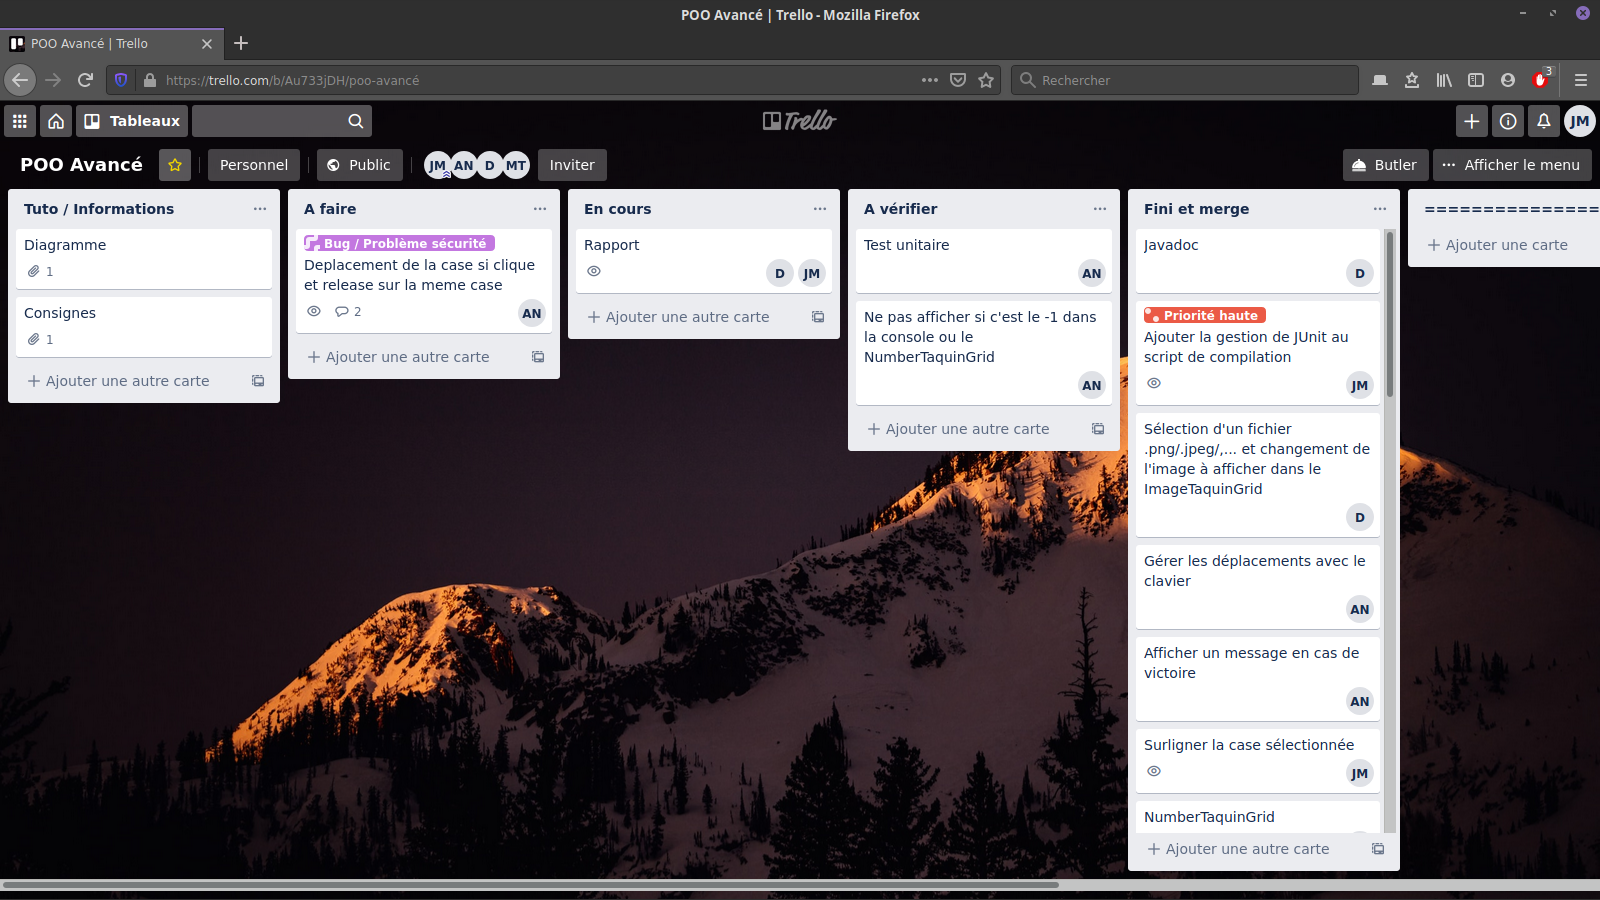
\includegraphics[width=0.75\textwidth, keepaspectratio]{img/trello.png}
				\caption{Notre tableau Trello}
				\label{fig:trello}
			\end{figure}

			Ainsi, comme nous pouvons le constater, les différentes tâches passent par différents états, "\textit{A faire}", "\textit{En cours}", "\textit{A vérifier}", "\textit{Fini et merge}". Enfin, bien que ce ne soit pas visible sur l'image \ref{fig:trello}, il existe un "\textit{Backlog}" sur la droite qui contient les différentes tâches restantes à accomplir. Celles-ci peuvent ensuite être déplacées dans la colonne "\textit{A faire}" au moment où nous jugeons qu'elles peuvent être réalisées.

			Les colonnes "\textit{A verifier}" et "\textit{Fini et merge}" nécessitent quelques précisions, les autres parlant d'elles-même. Pour la première, lorsqu'une tâche est terminée, elle est soumise à évaluation et relecture. Cela permet d'obtenir un avis sur la fonctionnalité et d'éviter d'éventuels bugs par la suite mais aussi de garder une cohérence au travers du code. Raisons pour lesquelles les personnes qui effectuent cette relecture sont souvent les mêmes. Enfin, quand celle-ci est vérifiée et validée, nous pouvons alors la déplacer dans la seconde colonne.

		\subsection{Discord}

			Afin de faciliter la communication au sein du groupe, nous avons utilisé le service de messagerie \href{https://discordapp.com}{Discord} car tous les membres du groupe l'utilisaient déjà de manière personnelle. Celui-ci permet de parler par le biais de "serveurs" gratuits dans lesquels nous pouvons ajouter des salons textuels ou des salons vocaux à volonté. Ainsi, nous avons deux salons de discussion. L'un nommé "\textit{important-taquin}" permet de transmettre des messages importants sur ce qui a été fait, sur des changements importants concernant le projet, etc. L'autre se nommant "\textit{dev-taquin}", est une discution beaucoup plus générale dans laquelle on peut demander de l'aide, aider des membres en difficulté, ou même de discuter de certains choix à faire.

			\begin{figure}[H]
				\centering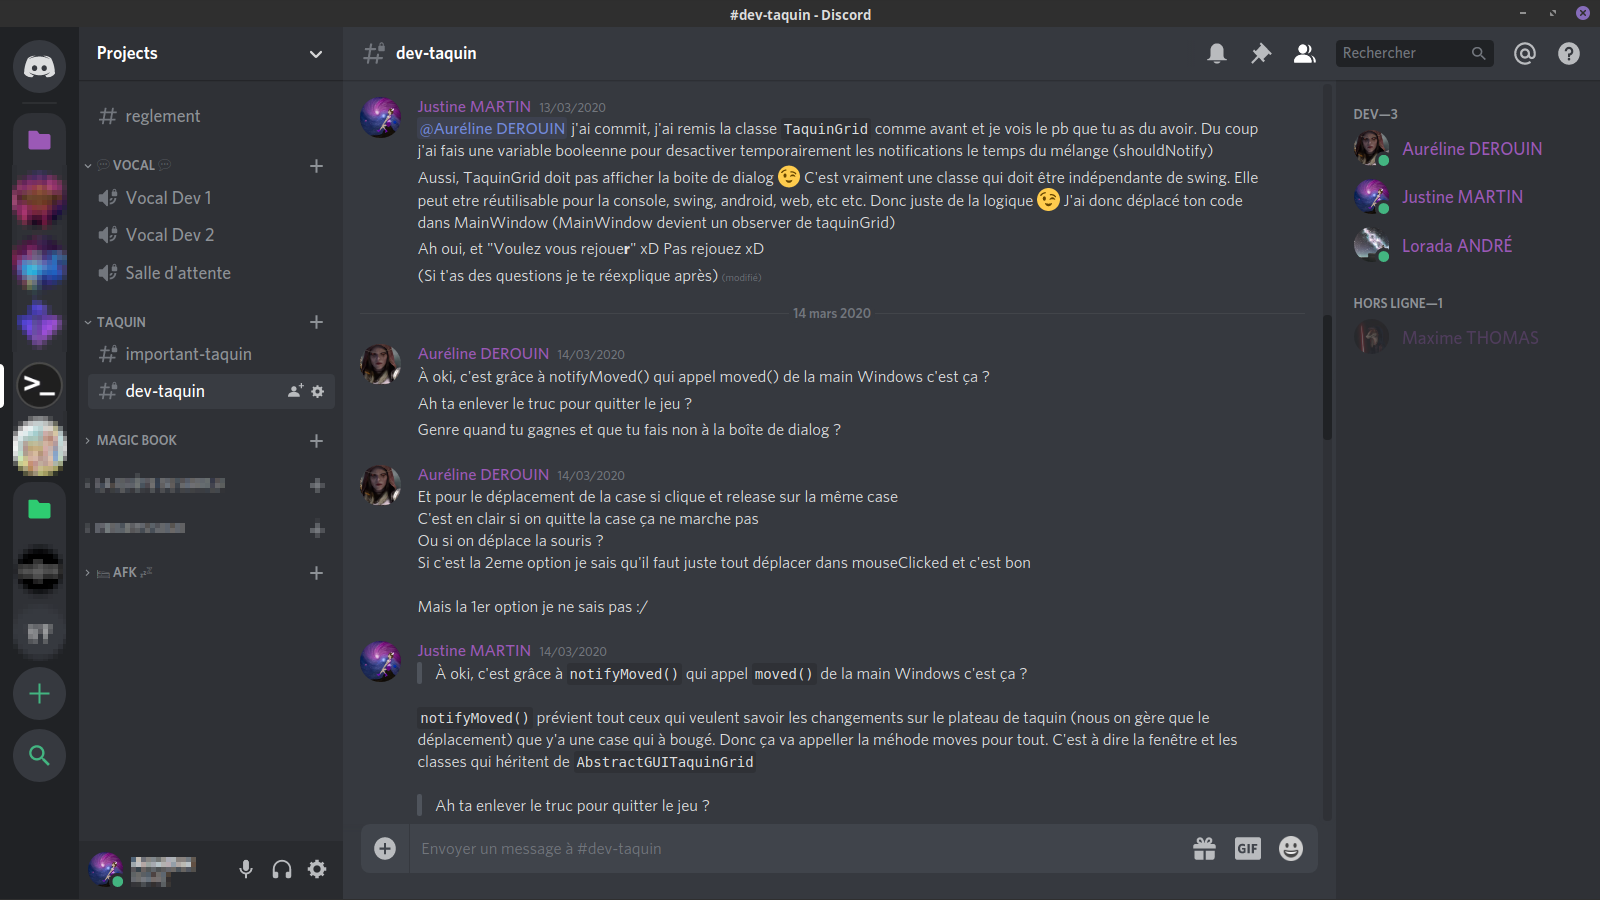
\includegraphics[width=0.75\textwidth, keepaspectratio]{img/discord.png}
				\caption{Notre serveur Discord}
			\end{figure}

	\section{Répartition des fonctionnalités}

		\begin{figure}[H]
			\begin{center}
				\begin{tabular}{l l}
				\multirow{7}{4em}{Auréline DEROUIN}
					& - Vue-Contrôleur du taquin avec les numéros (fenêtre)\\
					& - Classe Modèle du taquin\\
					& - Évènements clavier\\
					& - Énum Direction\\
					& - Afficher un message en cas de victoire (fenêtre)\\
					& - Tests unitaires\\
					& - Rapport\\
				 & \\

				\multirow{9}{4em}{Justine MARTIN}
					& - Vue-Contrôleur du taquin avec une image\\
					& - Vue-Contrôleur en mode console\\
					& - Évènements souris\\
					& - Mettre en évidence la case déplaçable\\
					& - Déplacement des cases avec la souris\\
					& - Boite de dialogue (classe mère et dialogue de nouvelle partie)\\
					& - Script build.sh\\
					& - Javadoc (relecture et précisions seulement)\\
					& - Rapport\\
				 & \\

				\multirow{6}{4em}{Lorada ANDRE}
					& - Gestion de la fenêtre principale (conception, menu, événement, etc)\\
					& - Gestion des arguments dans la Main\\
					& - Sélection et changement de l'image à afficher sur le taquin\\
					& - Javadoc\\
					& - Commande pour zipper dans build.sh\\
					& - Rapport\\
				 & \\

				\multirow{3}{4em}{Maxime THOMAS}
					& - Classe Modèle du taquin\\
					& - Interfaces pour le Pattern Observer\\
					& - Remélange le taquin si une fois mélangé, il est déjà complété\\

				\end{tabular}
			\end{center}
		\end{figure}
